\documentclass[11pt]{article}
\setlength{\topmargin}{-.2in}
\setlength{\oddsidemargin}{-0cm}
\setlength{\evensidemargin}{-1cm}
\setlength{\textwidth}{16.3cm}
\setlength{\textheight}{22.3cm}
\usepackage{graphicx}
\usepackage{subfigure}
\graphicspath{{figures/}}
\usepackage[round]{natbib}
\title{Effects of Irregular Topology in Non-Planar SOM Variants}
\author{\sc{Charles R. Schmidt}\\Regional Analysis Laboratory\\Department of Geography\\San Diego State University}
\date{\today} %\date{January 29th, 2007}
\begin{document}
\maketitle
\begin{abstract}
The development of the spherical SOM has been driven by the border effects
observed in traditional SOM.  Two problems exist with the Spherical SOM. The
first is the level of control over the network size. The second is the
topologically induced errors caused by the arrangement of neurons on the sphere.
Both of these problems stem from the problem of uniformly distributing points on
a sphere. These problems will be investigated through the introduction of a new
method for testing topologically induced errors. The method first analyzes  the
neural network to find topological mis-matches, next we train the network with
an overwhelming about of synthetic data.  Through a series of simple plots we
can then compare each neurons internal variance as defined by the variance of
the observations that best fit that neuron with suchs metrics as neighborhood
influence, number of child observations, etc.
\end{abstract}


%\section{Problem Statement}
%1. Introduction (10\%)
%\\2. Background and Lit Review (30\%)
%\\	\ldots Problem Statement
%\\	\ldots Lit Review
%\\3. Research Design / Plan / Metodology (50\%)
%\\4. Significance and Limitations (10\%)
%\\5. Timetable

\section{Introduction}
Using a spherical lattice is widely suggested as a solution to the boundary
effect found in the traditional Self-Organizing Maps \citep{ritter99, boudjemai2003,
sangole03, wu2006, Nishio:2006fk}.  However, the use of the spherical lattice
introduces a new problem.  Save the five platonic solids, distributing points on
a sphere will always result in irregular topology \citep{ritter99}.  The classic
method for generating a spherical lattice is to tessellate the sides a platonic
solid.  When tessellating the icosahedron, as described by \cite{wu2006}, the
resulting topology will always consist of \(12\) pentagons and \(N-12\) hexagons.
Where \(N\) is the total number of sides, or neurons.  The main drawback of this
method is the finite control over \(N\), which grows at a rate of \(f^2*10+2\),
where \(f\) is the frequency of the tessellation \citep{wu2006}.  There has been
little discussion on the effects of irregular topology in Spherical SOM. The goal of
this research is to investigate these effects in order to determine the usefulness of
slightly more irregular topologies which offer greater control over \(N\).

\section{Background and Lit Review}
The Self-Organizing Map (SOM) is an unsupervised competitive learning process
developed by Teuvo Kohonen as a technique to analyze high dimensional data sets.
The SOM algorithum uses an artificial neural network to organize high
dimensional data onto a low dimensional lattice, or map, of neurons.  Each
neuron contains a reference vector that can be considered to model a portion of
the input space. Before training these neurons are initialized, most commonly to
random values.  During the training process a randomly selected input vector
searches the map for its best matching unit (BMU), that is the neuron to which
it is most similar. The BMU and its neighborhood, as defined by a neighborhood
function, are than adjusted to better match that observation
\citep{Kohonen2000}.  The training process is repeated a predefined number of
times, or ideally until the map converges.  The traditional SOM is laid out on a
two dimensional plane using either a rectangular or hexagonal topology.
According to \cite{wu2006} the hexagonal structure is more uniform and
generally preferred.

\subsection{Boundary Effect}
\begin{figure}
\centering
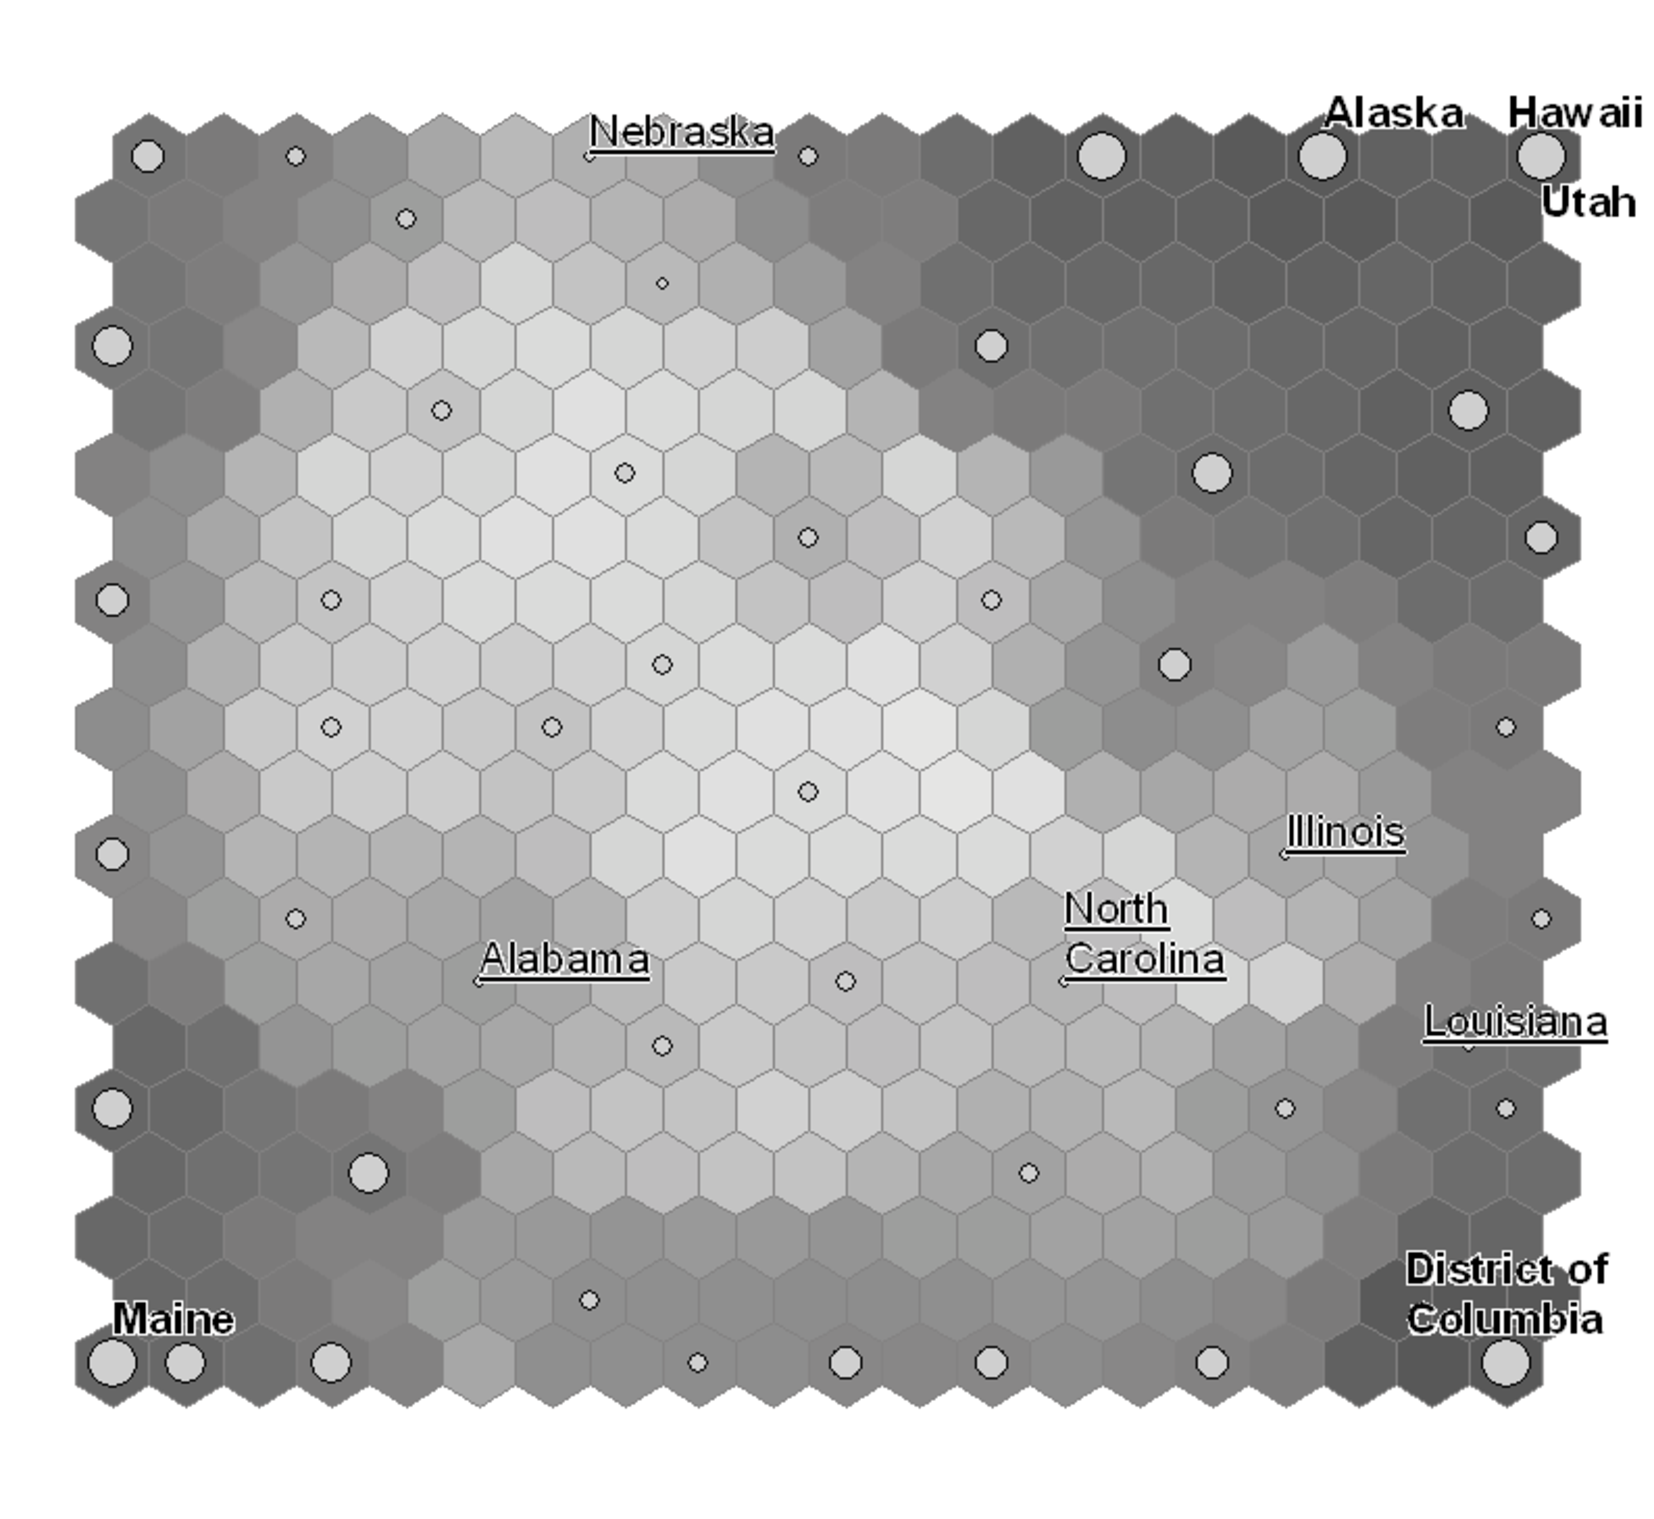
\includegraphics[width=1\linewidth]{gridedge_grey.pdf}
\caption{Fifty states plus D.C. mapped onto SOM trained with the first
thirty-two census variables.  Darker neurons have a relatively large differences
from the mean of the states, while lighter neurons are relatively closer.
Larger dots represent inputs that were poorly fit to the map, small smaller dots
show inputs that were better bit to the map.}
\label{figure1}
\end{figure}

One obvious drawback of building the neural lattice in a discrete euclidean
plane is the boundary of the resulting lattice.  A neuron located on the boundry
has fewer neighbors and thus fewer chances of being updated \citep{wu2006}.  As
observed in Figure \ref{figure1}, neurons in the center of the map tend to
better represent the mean of the input-space.  This is arguably caused by
outliers being pushed to the edges of the map, where they encounter fewer
competing signals.

The toroidal som was introduced by \cite{li1993} and removes this drawback.
However, the torus is not hugely effective for visualization, as maps generated
from a torus are not very intuitive \citep{ito2000,wu2006}.  \cite{ritter99}
describes the torus as being topologically flat and suggests that a curved
topology, such as that of a sphere, may better reflect directional data.  A
sphere also results in a more intuitive map, since we are accustomed to looking
at maps based on a sphere.

\subsection{Spherical SOM}
\cite{ritter99} first introduced the spherical SOM and several enhancements have
since been suggested \citep{boudjemai2003,sangole03,Nishio:2006fk,wu2006}.  A
good comparison of these enhancements can be found in \citep{wu2006}.  All of
these methods derive their spherical structure through the tessellation of a
polyhedron as originally proposed by \citeauthor{ritter99}.  \cite{wu2006} point
out the importance of a uniform distribution on the sphere and that it is
preferable for all neurons to have an equal number of neighbors and to be
equally spaced.  They find generally that the tessellation method best satisfies
these conditions and specifically that the icosahedron is the best starting
point \citep{wu2005}. Tessellation of the icosahedron results in a network of
neurons, each of which have exactly six neighbors, save the original twelve which
each have five.  This is very close to the ideal structure in which every neuron
would have exactly six neighbors.  This structure has very low variances in both
neuron spacing and neighbor size.  

\subsection{Network Size}
%Add background material on why Network Size is important.  The need for big and small networks.
%Waiting for Kohonen Book!!!	
The literature offers little theoretical guidance on network size
\citep{cho1996}.  \cite{toolbox} suggests simply using a network size of
\(5*\sqrt {n}\), where \(n\) is the number of observations.  The tessellation
method used by the class of spherical SOMs based on Ritter's work results in a
network size that is a function of the tessellation frequency and therefore
grows exponentially. In practice 2D Euclidean SOMs also offer limited control
over network size, as it is undesirable to have one dimension dramatically
larger then the other.  \cite{Nishio:2006fk} try to address the issue of network
size granularity by departing from the tessellation method and suggesting the
use of a partitioned helix to uniformly distribute any number of neurons on a
sphere.  A similar method was dismissed by \cite{wu2005} for failing to satisfy
the uniformity conditions.  \citeauthor{Nishio:2006fk} seem to have addressed
variance in nearest neighbor distances, but the issue of having a uniform number
of direct neighbors is still not addressed.

\subsection{Uniformity}
%\subsubsection{Neuron Spacing and Neighborhood Size Variance}
\citeauthor{wu2006} state that ``[f]or SOM, it is desirable to have all neurons
receive equal geometrical treatment'' \cite[pp. 900]{wu2006}.  To satisfy this
constraint two conditions must be met.  Firstly, each neuron should occupy the
same amount of space on the given surface.  Secondly, each neuron should be
bordered by the same number of surrounding neurons, and we should maximize 
that number.  The first condition in hugely important for visualization, but 
irrelevant for training.  During the training of the SOM only the topology of the 
neurons is considered.

Based solely on measures of neuron spacing \cite{wu2005} dismissed a method
proposed by \cite{Rakhmanov94} for distributing points on a sphere.  Similarly
\cite{Nishio:2006fk} use these variance measures to support their helix
algorithm for distributing points on a sphere.  Table \ref{table1} shows that
these metrics can be misleading and may not be comparable across topologies.
The traditional rectangular and hexagonal topologies have no variance in neuron
spacing and the generally preferred hexagonal structure displays greater
variance in neighborhood size than the rectangular structure.  The torus by
comparison would have variance in neuron spacing, yet no variance in
neighborhood size.  The distance between two neurons is only considered during
the formation of the neuronal network.  At this stage the spacing is significant
as it plays a part in determining neuron adjacency. However using this measure
to evaluate potential topologies for use in SOM may be misleading.

\begin{table}[htbp]
\caption{Variances in Topologies}
\begin{center}
\begin{tabular}{|c|c|c|c|}
\hline
Topology&Grid Size&Neuron Spacing&Variance in Neighborhood Size\\
\hline
Rectangular&9x18&1&0.2716\\
Hexagonal&9x18&1&1.2138\\
Tessellation&162&0.25319 - 0.31287& 0.0686\\
Rakhmanov&162&0.15779 - 0.30069& 0.2908\\
\hline
\end{tabular}
\end{center}
\label{table1}
\end{table}

Methods, for distributing points on the sphere, which allow for fine grained
control over network size produce slightly more irregular topologies.  However,
no discussion of these irregularities or their effects on SOM training has
occurred in the literature. Given that limited theoretical guidance is available
for choosing network size the desire for finer control over the network size,
should not be overlooked. In particular for a larger SOM the ideal network size
may not be achievable via tessellation of the icosahedron.

\section{Data and Methodology}
It is useful to represent our neural lattice as a graph, G.
We know that any arrangement of neurons onto the surface of a sphere will 
 as such the network can be effectively treated as a graph.  Doing so enables us to use the properties of the graph and the principles of graph theory to help us understand the relationship between neurons during training.


%%
%% ....
%%



the variance in neuron spacing should be minimized.    The first condition ensures that each neuron will occupy is only of concern when visualizing the SOM.



The get at the second condition we must first define the degree of a neuron, deg(n) to be number of its direct neighbors.  Whit that in mind the second condition is that the variance in the degree of the neurons must also be minimized.


This statement may be somewhat misleading to those investigating alternative 


For the purpose of SOM visualization it is important for each neuron to receive equal geometrical treatment.


It is useful to represent the neural network as a graph, G, in order use the...
In order to examine the irregularites in the neural network it is useful ....



The basic problem of the "boundary effect" is that neurons on the edge have
fewer neighbors. Yet there are only five possible arrangements of points on a
sphere such that all points have the same number of neighbors.  Any spherical
lattice consisting of more then twenty (dodecahedron) neurons will contain
topological irregularities.  This is to say that not all neurons will have the
same number of neighbors.  The importance of these irregularities and the 
magnitude of their effects on SOM training is not known.  This goal of this research
is to determine whether more flexible network structures may be used in spherical 
in SOM without introducing significant errors. To accomplish this goal, basic methods 
in network analysis with be combined with the result from several empirical training
runs each utilized different topology.  

\subsection{Synthetic Data}
In order to have a basis for comparison 


\bibliographystyle{apalike}
\bibliography{som}
\end{document}
